% id: 143-19
% book: 베이직쎈 대수 · 08 삼각함수의 활용
% section: 유형 084 사인법칙과 코사인법칙의 실생활에의 활용
% figure: tikz:fig-143-19
% answer: 
% answer_source: 
% variant_level: 0 (원본 전사)
% 이 파일은 build.mjs 가 items.json 에서 만든다. 고칠 때는 items.json 을 고친다.
\smash{\raisebox{1.5mm}{\dmkichul{베이직쎈 대수 143쪽 19번}}}
\noindent\begin{minipage}[t]{0.58\linewidth}\vspace{0pt}\raggedright 오른쪽 그림과 같이 $40\mkern3mu \mathrm{m}$ 떨어진 두 지점~$\pt{A}$, $\pt{B}$에서 비행 중인 비행기를 올려다본 각의 크기가 각각 $75^\circ$, $60^\circ$이었다. 이때 $\pt{A}$ 지점에서 비행기까지의 거리는?\end{minipage}\hfill\begin{minipage}[t]{0.4\linewidth}\vspace{0pt}\centering \resizebox{\ifdim\width>\linewidth\linewidth\else\width\fi}{!}{% 143-19(143쪽) — 지면 위 40 m 떨어진 두 지점 A, B 에서 비행 중인 비행기를 올려다본 각 75°·60°.
% 스캔 삽화(비행기 그림·흙바닥 무늬)는 화질이 낮아 TikZ 로 기하만 다시 그렸다.
% 라벨은 원문에 있는 A·B·75°·60°·40 m 만 두고 A 지점에서 비행기까지의 거리(답)는 적지 않는다.
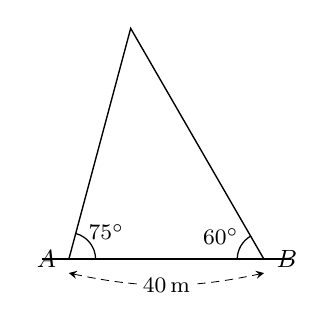
\begin{tikzpicture}[scale=0.62, line width=0.5pt, >=stealth]
  \coordinate (A) at (0,0);
  \coordinate (B) at (4,0);
  \coordinate (P) at (1.268,4.732);
  \draw[line width=0.7pt] (-0.55,0) -- (4.55,0);
  \draw (A) -- (P) -- (B);
  \draw[line width=0.45pt] ([shift=(0:0.55)]A) arc (0:75:0.55);
  \draw[line width=0.45pt] ([shift=(180:0.55)]B) arc (180:120:0.55);
  \node[font=\footnotesize] at ([shift=(36:0.95)]A) {$75^\circ$};
  \node[font=\footnotesize] at ([shift=(152:1.0)]B) {$60^\circ$};
  \node[left=1pt, font=\small] at (A) {$\pt{A}$};
  \node[right=1pt, font=\small] at (B) {$\pt{B}$};
  \draw[densely dashed, line width=0.3pt, <->] (0,-0.28)
    to[bend right=12] node[midway, fill=white, inner sep=1pt, font=\footnotesize] {$40\,\mathrm{m}$} (4,-0.28);
\end{tikzpicture}
}\end{minipage}\par
\begin{choicesii}{\rule[-3ex]{0pt}{8ex}$20\sqrt{2}\mkern3mu \mathrm{m}$}{\rule[-3ex]{0pt}{8ex}$30\mkern3mu \mathrm{m}$}{\rule[-3ex]{0pt}{8ex}$20\sqrt{3}\mkern3mu \mathrm{m}$}{\rule[-3ex]{0pt}{8ex}$36\mkern3mu \mathrm{m}$}{\rule[-3ex]{0pt}{8ex}$20\sqrt{6}\mkern3mu \mathrm{m}$}\end{choicesii}
